\chapter{INTRODUCTION}

The purpose of this chapter is to introduce \emph{Scandal}, a \emph{Java} framework and domain-specific language designed to process sounds and compose music. Computer music languages and applications have a long and established tradition, dating back to the late Fifties. Even though mainstream commercial music is mostly produced with graphical user interface tools nowadays, these tools are not adequate for audio signal processing with the specific intent of creating art music. The specificity of these tools render them inflexible to artistic extrapolations which lie at the heart of creative activity. Programming languages are still ubiquitous among art musicians and digital artists in general, and will likely remain so, given the flexibility artistic creation requires.

More specifically to audio and music, three domain-specific languages are used by the vast majority of art musicians, namely \emph{Csound}, \emph{Max}, and \emph{Supercollider}. All three are very mature tools, the youngest being \emph{Supercollider}, with over 20 years of development. All three impose a rather steep learning curve to musicians in general, and are commonly the subject of graduate coursework in music composition. Being that these DSL's are fairly high-level languages, they inevitably hide implementation details in a fashion that is often more useful for the seasoned developer that it is for the aspiring artist. In that regard, it is sometimes difficult to \emph{teach} the fundamentals of digital audio using these tools directly, for what they hide is often invaluable to understanding the inner workings of audio signal processing. While beneficial, learning a lower-level implementation \emph{first} is not at all the current practice among musicians.

\emph{Scandal} is a tool that aims at filling this gap by exposing the end user to some of the implementation details of digital audio, while remaining a fairly high-level language. In fact, a \emph{Scandal} program may be as high level as is adequate for the end user. At the same time, a \emph{Scandal} program is capable of exposing to the programmer the direct mathematical manipulation of each sample in an audio buffer using the exact same language constructs that lower-level languages do, that is, conditional and control statements, variable declarations, and methods. As a design choice, however, \emph{Scandal} is not object-oriented, exactly because its DSL is meant as a pedagogical tool, and the OOP paradigm is already a level of abstraction above most scripting languages. On the other hand, a plain scripting language is usually very imperative, and signal processing in general benefits from declarative constructs, especially those whose constituent parts can be modularized and reorganized, as to simulate specialized boxes within a signal flow. In order to have these qualities, without the overhead of being object-oriented, \emph{Scandal} was designed to be a scripting language with non-pure functional capabilities. A pure functional language would have been too abstract for the learner, however \emph{Scandal} emphasizes its functional qualities very obnoxiously. As the next section demonstrates, the \emph{only} way a method can be declared in \emph{Scandal} is as a lambda expression.

The expected result of this thesis is the proof-of-concept of a language implementation that can handle arbitrary audio signal processing algorithms and algorithmic music composition. Naturally, the language implementation will be incomplete to some extent, but this document shall provide the basic foundation to completing the language implementation in the future. Moreover, no single tool should ever be expected to cover all possible applications of audio signal processing and music composition, hence \emph{Scandal} is limited in that it requires being used in conjunction with other technologies and programming languages. Reading this document requires a working knowledge of how programming languages are defined in terms of their concrete and abstract syntaxes, as well as a basic knowledge of how compilers work, from tokenizing an input to generating target code, including a working knowledge of top-down, recursive descent parsers. It is assumed that the reader will have knowledge of basic algorithms and data structures, such as stacks and binary trees. Being conversant in one or more general-purpose programming languages is advisable. In addition, the reader is expected to have some, but very little, background in digital signal processing. A background in music is not required, but highly desirable.

\section{A Tour of \emph{Scandal}}

In a nutshell, \emph{Scandal} is a compiled scripting language with a functional flavor. Its types are static and declared explicitly. A single exception applies to the lambda type, which is a parameterized type, and whose parameter types are inferred. At the topmost level of a \emph{Scandal} program, there are basically only two kinds of constructs that are allowed, namely declarations and statements. The legal declarations at this level are further subdivided into three: assignment declarations, field declarations, and lambda literal declarations. There is a fourth type of declaration, the parameter declaration, that is not allowed as a top-level construct. It follows every variable declaration in \emph{Scandal} must be initialized, except when they are parameters of a lambda literal, in which case they actually cannot be initialized. Even blocks are not allowed on their own, and may only occur in the context of a conditional or control statement, or of a lambda literal expression. Listing \ref{alg:finder} provides an example of the imperative side of \emph{Scandal}.

\begin{lstlisting}[emph={int,bool,while,if,true,false,print},emphstyle={\textbf},caption={A naive algorithm to determine whether an integer is prime.},label={alg:finder}]
int p = 571
int q = 2
bool result = true
while (q < p) {
	if (p % q == 0) {
		result = false
		q = p
	}
	q = q + 1
}
print(result)
\end{lstlisting}

\emph{Scandal} supports a handful of types that are built into the language, however user-defined types are not supported as of yet, but certainly planned. The built-in types are integers, floats, booleans, arrays of floats, strings, and lambdas. Integer an boolean literals are declared as usual, and float literals are declared the same way \emph{Java} doubles are, without a trailing \il{f}. String literals are declared with double quotes only, and single-quote characters are not part of the language. Array literals are declared as comma-separated expressions surrounded by brackets, like \il{array a = [1, 2, 3]}, and their entries retrieved with a name followed by an index surrounded by brackets, like \il{a[0] = 4}. Indexed arrays in \emph{Scandal} must have the array necessarily bound to a name, and an expression like $[1, 2, 3][0] == 1$ is not allowed. Array items can be integers or floats, but the array will ultimately contain only floats. Such an array as \il{array b = [1, pow(2, 3.2), 3.5, pi]} would be perfectly legal. \emph{Scandal} features type polymorphism between integers and floats, and in many but not all situations these types can be used interchangeably. Arithmetic operators are \emph{ad-hoc} polymorphic, and many built-in functions feature type coercion. Lambda applications, on the other hand, do not feature parametric type polymorphism. Integers and booleans, or floats and booleans for that matter, cannot be used interchangeably in \emph{Scandal} at all. Numbers and booleans can, however, be combined in logical and comparative binary expressions, where operators are overloaded.

\subsection{Input/Output Operations}

Given that \emph{Scandal} is geared toward audio signal processing and electro-acoustic music composition, the language provides a few hard-wired routines that are aimed at facilitating common operations in the language's domain. These are namely importing, capturing, and playing back audio files, as well as plotting arrays as graphs and printing expressions to the console. In addition, a variety of mathematical constants and functions are easily accessible everywhere in the language, such as transcendental functions and pi, for example.

Importing audio files in \emph{Scandal} is straightforward, and all that is needed is a \il{read} statement and a string pointing to the path of a \emph{.wav} file in the file system. Visualizing array data is also simple with a \il{plot} statement. Playback is performed in real time and set to loop indefinitely, despite the length of the audio buffer. Therefore, for all but very few applications, there should be a single \il{play} statement per \emph{Scandal} program, since each \il{play} statement initiates a new audio thread. Playback threads are always different from the thread in which the compiler runs, which in turn is a separate thread from the main user interface thread. Hence multiple \il{play} statements will sound simultaneously.

Unlike \il{play}, \il{record} captures from the default audio input by blocking the compiler thread, so that no playback in a given program occurs simultaneously with a recording. Of course, other programs may be playing back in different threads. Listing \ref{alg:inout} exemplifies the input/output functionality of \emph{Scandal}. %An implementation of \emph{I Am Sitting in a Room}, for example, might require two different \emph{Scandal} programs running at the same time on the IDE.

\begin{lstlisting}[emph={array,read,string,plot,print,record,play,import},emphstyle={\textbf},caption={Inputting and outputting in \emph{Scandal}},label={alg:inout}]
array lisa = read("wav/monoLisa.wav", 1)
plot("A Scandalous Sound File", lisa, 1000)

print("Recording...")
array recording = record(10000)

print("Playing...")
play(recording, 1)
play(lisa, 1)
\end{lstlisting}

\begin{enumerate}
	\item Lines 1 and 2 simply import the audio file in the given path and open a plot tab in the IDE, decimating the length of the plot to 1000 points.
	\addtocounter{enumi}{2}
	\item Line 4 prints to the console a message to inform the user that recording has started, and line 5 saves ten seconds of captured audio data into an audio buffer. For the duration of the recording, the execution thread will be blocked, and none of the subsequent statements will be executed.
	\addtocounter{enumi}{2}
	\item Line 7 will print to the console that playback has begun, and line 8 starts a real-time audio thread that plays the captured audio back. Since every \il{play} statement runs on its own thread, none of them block the execution thread, and the statement in line 9 will play back simultaneously with the one in line 8.
\end{enumerate}

\begin{figure}[p]
	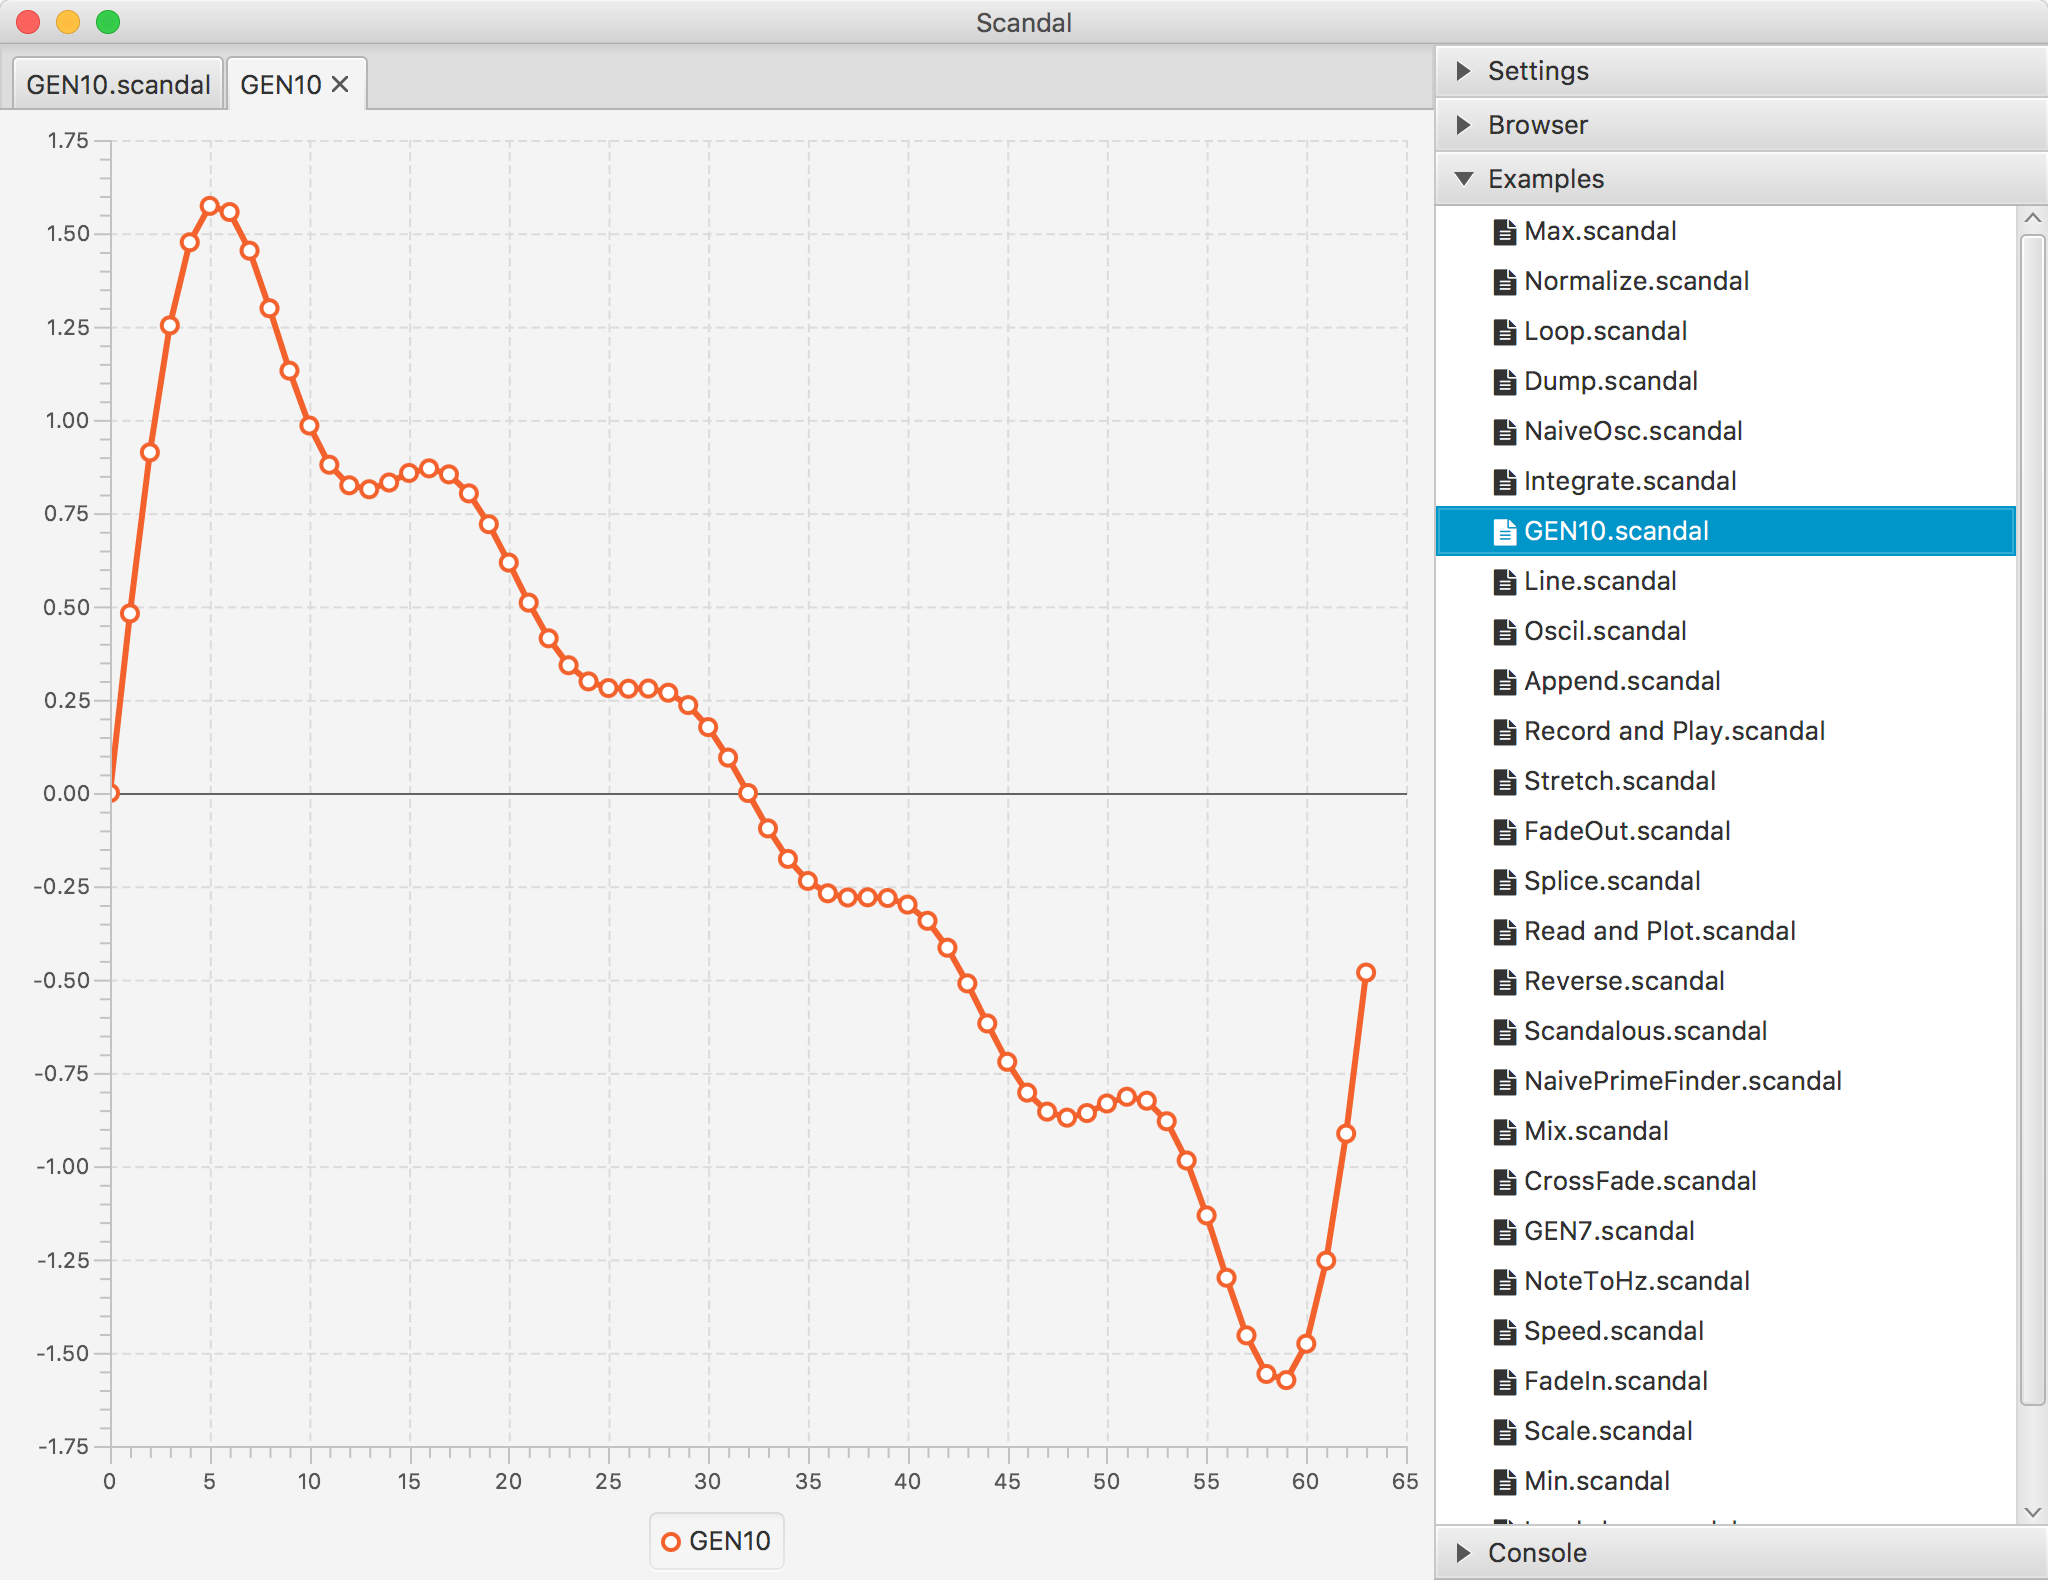
\includegraphics[width=4.5in]{img/plot}
	\caption[Plotting an array in \emph{Scandal}.]{Plotting an array in \emph{Scandal}.}
\end{figure}

\clearpage

Even though the language \emph{can} behave in the imperative fashion exemplified above, a lot of effort has been put into making it as declarative as possible. In fact, expressions in \emph{Scandal} cannot be evaluated at all on their own, rather existing only in the context of a declaration or statement, contrary to many languages that will allow expressions to be evaluated directly on the command line. \emph{Scandal} can work on the command line, but some of its functionality is restricted there. Namely, plots are not shown, and the playback thread blocks, that is, it is impossible to hear two \il{play} statements simultaneously. To mitigate the imperative impulse of a scripting language, \emph{Scandal} proposes the use of lambda expressions, which will be discussed later in this chapter. In effect, one can compose an entire piece of music in \emph{Scandal} practically with lambda expressions alone. These lambdas can be broken down into partial applications of their constituent parts, and those can in turn be composed with other lambdas, providing the language with great flexibility. The next sections present a sampler of \emph{Scandal} implementations of some general-purpose algorithms, with a focus on the language's limitations, which are natural, given the specificity of its domain of applications. Many of the programs discussed here come bundled with \emph{Scandal}'s IDE, under the \emph{Examples} tab of its right accordion view.

\subsection{Array Operations}

Much of audio signal processing relies on some very general array operations. Among these, modifying the amplitude of an audio signal boils down to simply multiplying a vector by a scalar, the latter usually between zero and one. Changing the dynamics of an audio buffer is often an algorithmic task, and audio engineers have at their disposal a large palette of techniques which ultimately consist of applying scalars to buffers of audio data. Such techniques include compressing, expanding, limiting, dithering, and normalizing. Normalizing a buffer of audio data is extremely simple, as the scalar is just the multiplicative inverse of the maximum element in the array. Since audio samples are usually represented by floats ranging from minus one to one, care must be taken when testing for the maximum array element, for it could be a negative value. When samples are allowed to take negative values, the absolute value of every sample must be considered, otherwise the result might not be a normalized array (whose maximum element is one). Listing \ref{alg:max} describes finding an array's absolute maximum in \emph{Scandal}.

\begin{lstlisting}[emph={lambda,array,float,int,while,size,if,return},emphstyle={\textbf},caption={Computing the maximum element of an array.},label={alg:max}]
lambda max = array x -> {
	float m = x[0]
	float sample = 0
	int i = 0
	while i < size(x) {
		sample = x[i]
		if sample < 0 { sample = -sample }
		if m < sample { m = sample }
		i = i + 1
	}
	return m
}
\end{lstlisting}

Listing \ref{alg:max} is very straightforward to understand. Given that there are no for-loops in \emph{Scandal}, one must declare an induction variable outside the while-loop, then increment it inside the loop's block. At the moment, there is no \il{abs} operator either, and computing the absolute value in line 7 can certainly be improved by refactoring that line into another lambda, which could in turn be made available for later use. Rather than bloating the compiler with dozens of mathematical expressions, the preferred avenue is to allow for the language to evolve in terms of itself, and only functions that are more difficult to compute, such as trigonometric functions, are being hard-wired to the compiler at this point.

In the spirit of making \emph{Scandal} code as reusable as possible, the normalization procedure makes use of a \il{scale} lambda whose parameters are an array to be scaled, and a function that determines a scalar in terms of the array itself. The implementation of \il{scale} is straightforward and thus omitted. The idea is to apply to \il{scale} both an array, and a function that computes the multiplicative inverse of the array's absolute maximum element. Then, multiplying each element of the array by its inverse maximum will effectively normalize it. For both improved performance and re-usability reasons, multiplications are preferred over divisions. Hence this design requires a function that computes the inverse maximum of an array. Listing \ref{alg:inverse} is a generic method that computes the reciprocal of \emph{any} lambda that takes an array and returns a float, such as \il{max}.

\begin{lstlisting}[emph={lambda,array,float,return},emphstyle={\textbf},caption={Computing the inverse of an \il{array -> float} lambda.},label={alg:inverse}]
lambda inverseLambda = array x -> lambda f -> {
	float val = f(x)
	return 1 / val
}
\end{lstlisting}

The value of \il{f(x)} in Listing \ref{alg:inverse} cannot be returned directly, as line 2 is crucial for the parameterized type inference mechanism of the compiler. It is because of line 2 that \il{inverseLambda} knows that it is a function that takes an array and a function, and returns a float. This parameter function is, in turn, a lambda that takes a single argument of type array and returns a float, hence \il{inverseLambda} itself must also return a float. The function \il{inverseMax} is the special case of \il{inverseLambda} that deals with computing the reciprocal of an array's maximum. Since lambda literals are always global, \il{inverseMax} could have been equivalently defined by substituting its return expression with the expression \il{1 / max(x)}, and dispensing altogether with \il{inverseLambda}. Normalizing a buffer of audio samples then becomes the single elegant line of \emph{Scandal} code given in line 2 of Listing \ref{alg:normal}. More than concise, the \il{normalize} method leaves all of its constituent parts, that is, every one of its different computational steps, open to be reused and recombined into other functions. That seemingly trivial characteristic of functional programming has in fact very deep implications to digital signal processing in general, and exploring its capabilities is one of \emph{Scandal}'s primary missions. The \emph{lib/Arrays.scandal} library included with the IDE contains many more examples of array operations in \emph{Scandal}, including routines to reverse and splice buffers of audio data.

\begin{lstlisting}[emph={lambda,array},emphstyle={\textbf},caption={Normalizing an array.},label={alg:normal}]
lambda inverseMax = array x -> inverseLambda(x, max)
lambda normalize = array x -> scale(x, inverseMax)
\end{lstlisting}

\subsection{An Overview of Lambda Expressions}

This section gives a brief overview of \emph{Scandal}'s functional capabilities. Listing \ref{alg:lambdas} summarizes the many syntactical constructs associated to lambdas in \emph{Scandal}, which are subsequently described, line by line. Lines 3 to 6 demonstrate currying, partial applications, and compositions; lines 8 to 10 show how literal lambdas may be copied into local or global variables; lines 12 and 13 show compositions may too be copied into local or global variables; lines 15 to 19 give an example of higher-order functions and their type-inference mechanism; finally, lines 21 to 26 demonstrate how lambda literals, applications, and compositions can capture the environment. 

\begin{lstlisting}[emph={field,float,lambda,return,print},emphstyle={\textbf},caption={The syntax of lambda expressions in \emph{Scandal}.},label={alg:lambdas}]
field float eleven = 11.0

lambda adder = float x -> float y -> x + y
lambda add4 = adder(4.0)
lambda add6 = adder(6.0)
float twentyOne = add6.add4(eleven)

lambda id = float x -> x
field lambda copy = id
eleven = copy(eleven)

field lambda copyComposition = add4.add6
twentyOne = copyComposition(eleven)

lambda higherOrder = float x -> lambda f -> {
	float val = f(x)
	return val
}
eleven = higherOrder(eleven, id)

lambda captureFloat = float x -> x + eleven
print(captureFloat(eleven))
lambda captureLambda = float x -> copy(x)
print(captureLambda(eleven))
lambda captureComposition = float x -> copyComposition(x)
print(captureComposition(eleven))
\end{lstlisting}

\begin{enumerate}
	\item The mechanism in \emph{Scandal} to capture the environment is to declare external variables as fields. Having been declared as such, \il{eleven} will be accessible inside lambda bodies.
	\addtocounter{enumi}{1}
	\item Functions that take multiple arguments are always curried in \emph{Scandal}. The declaration of \il{adder} is read ``adder is a lambda that takes a float \il{x}, that returns an anonymous lambda that takes a float \il{y}, that returns the expression \il{x + y}''.
	\item Applying arguments to a lambda expression fixes its parameters from left to right. Applying four to \il{adder}, fixes the parameter \il{x} and recovers the anonymous function defined by that parameter. Partial applications return functions, which can be freely stored for posterior use as applications or compositions.
	\addtocounter{enumi}{1}
	\item A lambda may be composed when its return type matches the input type of the lambda to its right. Here \il{eleven} is being applied to \il{add6}, which returns a float ($11 + 6 = 17$) that is fed to \il{add4}, which in turn returns another float ($17 + 4 = 21$) that is stored to \il{twentyOne}. At the moment, only copies of partial applications may be composed, that is, a lambda composition cannot have arguments preceding a dot. Function composition does not follow the mathematical notation $f \circ g(x) = f(g(x))$, in which $g$ is evaluated first. In \emph{Scandal}, functions are applied from left to right, as they are read, that is $f.g(x) = g(f(x))$.
	\addtocounter{enumi}{1}
	\item Literal lambdas can be copied to local or global (field) variables. The literal lambda \il{id} is always visible, and so is \il{copy}, since it was marked as a field.
	\addtocounter{enumi}{3}
	\item Copying compositions works the same way as copying any other lambda expression. Marking \il{copyComposition} as a field makes it visible inside lambda literal bodies.
	\addtocounter{enumi}{2}
	\item Higher-order functions are those that can take functions as arguments, return functions, or both. \emph{Scandal} supports higher-order functions, but it does not support parameterized types. In line 16, the parameter \il{f} needs to be given arguments before its result can be used in line 17, so that its input and return types may be inferred by the compiler. \emph{Scandal} still lacks the functionality of returning lambdas directly from function bodies. Lambdas can still return partial applications of themselves, though.
	\addtocounter{enumi}{5}
	\item When marked as fields, lambdas, as well as any other variable type, become available to every scope of a program. Line 21 demonstrates this behavior with a float, line 23 with a lambda, and line 25 with a lambda composition. Partial applications can be demonstrated the same way.
\end{enumerate}

At the moment, there is no simple mechanism to fix a parameter in the middle, given the enforced right-associativity of lambda expressions in \emph{Scandal}. There is, however, a workaround by declaring a new lambda literal that returns an application of the original lambda. The parameters in this new lambda literal are essentially the same, but reordered so that the fixed parameter is the leftmost, as seen in Listing \ref{alg:reorder}.

\begin{lstlisting}[emph={field,int,lambda,print},emphstyle={\textbf},caption={Right associativity of lambda expressions.},label={alg:reorder}]
field int w = 1
lambda f = int x -> int y -> int z -> x + y + z
lambda g = int x -> int z -> f(x, w, z)
\end{lstlisting}

\section{The Concrete Syntax of \emph{Scandal}}

This section provides a formal presentation of \emph{Scandal}, with rules for its concrete syntax. In the productions that follow, the star symbol represents a \emph{Kleene} star, and single-character symbols are not tokens in the language. As a rule, terminal symbols will be given by their names, like \texttt{OR}, to avoid confusion with symbols in the language's grammar. Terminal symbols are generally presented in the syntactical context in which they appear. In the discussions that follow, terminal symbols are in all-capital letters, productions in the concrete syntax begin with a lower-case letter, and their counterparts in the abstract syntax begin with an upper-case letter. Below are the production rules for top-level constructs.

\begin{itemize}
	\item program := (assignmentDeclaration $|$ fieldDeclaration)$^*$
	\item program := (lambdaLitDeclaration $|$ statement)$^*$
	\item assignmentDeclaration := types \texttt{IDENT} \texttt{ASSIGN} expression
	\item fieldDeclaration := \texttt{KW\_FIELD} types \texttt{IDENT} \texttt{ASSIGN} expression	
	\item lambdaLitDeclaration := \texttt{KW\_LAMBDA} \texttt{IDENT} \texttt{ASSIGN} lambdaLitExpression
	\item lambdaLitDeclaration := \texttt{KW\_LAMBDA} \texttt{IDENT} \texttt{ASSIGN} lambdaLitBlock
	\item types := \texttt{KW\_INT} $|$ \texttt{KW\_FLOAT} $|$ \texttt{KW\_BOOL} $|$ \texttt{KW\_STRING} $|$ \texttt{KW\_ARRAY} $|$ \texttt{KW\_LAMBDA}
	\item statement := importStatement $|$ assignmentStatement $|$ indexedAssignStat
	\item statement := ifStatement $|$ whileStatement $|$ printStatement
	\item statement := playStatement $|$ plotStat $|$ writeStat
	\item importStatement := \texttt{KW\_IMPORT} \texttt{LPAREN} expression \texttt{RPAREN}
	\item assignmentStatement := \texttt{IDENT} \texttt{ASSIGN} expression
	\item indexedAssignStat := \texttt{IDENT} \texttt{LBRACKET} expression \texttt{RBRACKET} \texttt{ASSIGN} expression
	\item ifStatement := \texttt{KW\_IF} expression block
	\item whileStatement := \texttt{KW\_WHILE} expression block
	\item block := \texttt{LBRACE} (assignmentDeclaration $|$ statement)$^*$ \texttt{RBRACE}
	\item printStatement := \texttt{KW\_PRINT} \texttt{LPAREN} expression \texttt{RPAREN}
	\item playStatement := \texttt{KW\_PLAY} \texttt{LPAREN} expression \texttt{COMMA} expression \texttt{RPAREN}
	\item plotStat := \texttt{KW\_PLOT} \texttt{LPAREN} expression \texttt{COMMA} expression \texttt{COMMA} expression \texttt{RPAREN}
	\item writeStat := \texttt{KW\_WRITE} \texttt{LPAREN} expression \texttt{COMMA} expression \texttt{COMMA} expression \texttt{RPAREN}
\end{itemize}

The concrete syntax rules for the various types of expressions are given in terms of binary expressions. The reason for defining them like so will become apparent in the next chapters when the construction of an abstract syntax tree is discussed. For now, every expression is defined in terms of a binary expression that has a left expression, a right expression, and an operator. Left and right expressions can be themselves binary expressions, of course, and operators may not exist at all, hence the Kleene star, so that a binary expression without an operator is simply its left expression. That is how trivial binary expressions are retrieved from the productions below. Seen as binary trees, trivial binary expressions are just single-leaf trees. The leaves are called factors in the production rules below. Above factors, there can be summands, and above summands there can be comparisons, depending on the precedence level of the connecting operators. In \emph{Scandal}, carets or double-stars are not allowed to denote exponentiation. Should them be allowed in the future, they would need to be introduced in the rules below with a higher precedence than factors, that is, powers would need to replace factors as leaves.

\begin{itemize}
	\item expression := comparison (comparisonOp comparison)$^*$
	\item comparisonOp := \texttt{LT} $|$ \texttt{LE} $|$ \texttt{GT} $|$ \texttt{GE} $|$ \texttt{EQUAL} $|$ \texttt{NOTEQUAL}
	\item comparison := summand (summandOp summand)$^*$
	\item summandOp := \texttt{PLUS} $|$ \texttt{MINUS} $|$ \texttt{OR}
	\item summand := factor (factorOp factor)$^*$
	\item factorOp := \texttt{TIMES} $|$ \texttt{DIV} $|$ \texttt{MOD} $|$ \texttt{AND}
	\item factor := derivedExpression $|$ literalExpression $|$ arrayExpression
	\item factor := frameworkExpression $|$ lambdaExpression
\end{itemize}

Derived expressions are those defined in terms of another expression. They exist in three contexts, namely when an expression is surrounded by parenthesis, when a number or boolean expression is negated, and as name references to other expressions. Below are the concrete rules for derived expressions.

\begin{itemize}
	\item derivedExpression := parethesizedExpression $|$ unaryExpression $|$ identExpression
	\item parethesizedExpression := \texttt{LPAREN} expression \texttt{RPAREN}
	\item unaryExpression := (\texttt{MINUS} $|$ \texttt{NOT}) expression
	\item identExpression := \texttt{IDENT}
\end{itemize}

Literal expressions are the simplest constructs in the language, since their values are not computed. They are naturally leaves in binary expression trees. Their concrete rules are very simple, and are given below.

\begin{itemize}
	\item literalExpression := intLitExpression $|$ floatLitExpression
	\item literalExpression := boolLitExpression $|$ stringLitExpression
	\item intLitExpression := \texttt{INT\_LIT}
	\item floatLitExpression := \texttt{FLOAT\_LIT}
	\item boolLitExpression := \texttt{KW\_TRUE} $|$ \texttt{KW\_FALSE}
	\item stringLitExpression := \texttt{STRING\_LIT}
\end{itemize}

In the productions above, non-zero integer literals are not allowed to have any number of leading zeros. The same applies to floating-point decimals, where only one zero may precede the dot. In this particular case, a zero actually \emph{must} precede the \texttt{DOT} token, and such constructs as $x = .5$ are not allowed. Doubles, shorts, or longs do not exist in \emph{Scandal} as of yet, and there is no need to declare float literals the way they are in \emph{Java}, with a trailing \il{f}. String literals are constructed by enclosing text within quotes, and the use of apostrophes will cause a scanning error. Even though quotes are in the language's alphabet, they are discarded upon conversion into tokens, as their only possible use is within a string literal. \texttt{DOT}, on the other hand, has uses besides separating the decimal part of a \texttt{FLOAT\_LIT}, namely in composed lambdas. Boolean literals are quite self-explanatory, and are not allowed to replace numbers in arithmetic expressions, as arithmetic operators are not overloaded to accept booleans. For all other operators, though, numbers and booleans can be used in the same expression. Also, unlike \emph{C}, numbers alone are not allowed to replace booleans in conditional and control statements.

Array expressions are fundamental to the DSL in that sound data is processed as arrays of floats. There are four types of array expression, namely literal array expressions, which are declared as comma-separated expressions surrounded by brackets, array items, which are floats retrieved from an array at a particular index, array sizes, which are integers corresponding to sizes of arrays, and lastly constructors of new arrays, which create arrays of zeros with a given integer size. Below are the concrete rules for the different types of array expressions.

\begin{itemize}
	\item arrayExpression := arrayLitExpression $|$ arrayItemExpression
	\item arrayExpression := arraySizeExpression $|$ newArrayExpression
	\item arrayLitExpression := \texttt{LBRACKET} expression (\texttt{COMMA} expression)$^*$ \texttt{RBRACKET}
	\item arrayItemExpression := identExpression \texttt{LBRACKET} expression \texttt{RBRACKET}
	\item arraySizeExpression := \texttt{KW\_SIZE} \texttt{LPAREN} expression \texttt{RPAREN}
	\item newArrayExpression := \texttt{KW\_NEW} \texttt{LPAREN} expression \texttt{RPAREN}
\end{itemize}

Framework expressions, like framework statements, provide functionality to \emph{Scandal} that would be impractical to implement in terms of the language alone. In some cases, though, they are just conveniences, like providing a keyword for the number pi. As discussed previously, this practice always imposes a trade-off, since by not allowing the language to grow in terms of itself, compiler bloat is inevitably experienced. Many framework statements and expressions will likely be bootstrapped into the language as it evolves. The primary difference between framework statements and expressions is that the latter return some value to be consumed. Below are the concrete rules for framework expressions.

\begin{itemize}
	\item frameworkExpression := piExpression $|$ cosExpression $|$ powExpression
	\item frameworkExpression := floorExpression $|$ readExpression $|$ recordExpression
	\item piExpression := \texttt{KW\_PI}
	\item cosExpression := \texttt{KW\_COS} \texttt{LPAREN} expression \texttt{RPAREN}
	\item powExpression := \texttt{KW\_POW} \texttt{LPAREN} expression \texttt{RPAREN}
	\item floorExpression := \texttt{KW\_FLOOR} \texttt{LPAREN} expression \texttt{RPAREN}
	\item readExpression := \texttt{KW\_READ} \texttt{LPAREN} expression \texttt{COMMA} expression \texttt{RPAREN}
	\item recordExpression := \texttt{KW\_RECORD} \texttt{LPAREN} expression \texttt{RPAREN}
\end{itemize}

\emph{Scandal} is not a pure functional language, however lambdas are the sole mechanism for defining methods in the language. Being that \emph{Scandal} is a statically-typed scripting language where new types are not explicitly defined, lambdas, as well as applications and compositions thereof, are in effect an essential part of the language in what regards encapsulation and code re-usability in general. As shall be seen in the next chapters, one can write an entire musical composition in \emph{Scandal} using only lambda expressions. There are four types of lambda expressions, of which two are literal. Literal lambda expressions differ from the other types in that they define a method body, either as a simple expression to be returned, or as an entire block, which in turn contains a return expression as its last statement. As previously discussed, literal lambda expressions, for the moment, are always global variables. They can nonetheless be copied into local variables, and accessed as such. The other two types are applications and compositions. The former has a familiar method-like syntax, with a name reference preceding comma-separated arguments surrounded by parenthesis. The latter has two possible uses, one where no arguments are given, in which the syntax consists of a list of name references connected by dots. The second use includes a list of arguments, and its syntax is that of a composition followed by a dot and an application. Below are the concrete rules for lambda expressions.

\begin{itemize}
	\item lambdaExpression := lambdaApp $|$ lambdaComp $|$ lambdaLit $|$ lambdaBlock
	\item lambdaApp := identExpression \texttt{LPAREN} expression (\texttt{COMMA} expression)$^*$ \texttt{RPAREN}
	\item lambdaComp := identExpression (\texttt{DOT} identExpression)$^*$
	\item lambdaComp := identExpression (\texttt{DOT} identExpression)$^*$ \texttt{DOT} lambdaApp
	\item lambdaLit := paramDeclaration \texttt{ARROW} (paramDeclaration \texttt{ARROW})$^*$ expression
	\item lambdaBlock := paramDeclaration \texttt{ARROW} (paramDeclaration \texttt{ARROW})$^*$ retBlock
	\item paramDeclaration := types \texttt{IDENT}
	\item retBlock := \texttt{LBRACE} (assignmentDeclaration $|$ statement)$^*$ retExpression \texttt{RBRACE}
	\item retExpression := \texttt{KW\_RETURN} expression
\end{itemize}